\chapter{Appuis, représentation et démarches}
\section{Appuis et liaisons}
	\subsection{Appuis usuels}
	Les trois appuis usuels sont ceux découverts au cours de \textit{Mécanique 
	rationnelle I}, à savoir l'appui à dilatation (rouleau), l'articulation et 
	l'encastrement.
	
		\subsubsection{Appuie à dilatation : rouleau}
		Le \textit{rouleau} permet le déplacement dans une direction ainsi que 
		la rotation. Ce genre d'appui est fréquent sous les ponts, souvent de 
		chemins de fer. En 2D, il possède une unique réaction de liaison, les 
		deux autres "mouvements" étant libres.
		
		\subsubsection{Articulation}
		L'\textit{articulation} permet la rotation mais sans déplacement. Il 
		possède deux réactions de liaisons, bloquant le déplacement.
		
		\subsubsection{Encastrement}
		L'\textit{encastrement} ne permet ni le déplacement, ni la rotation. En 
		bref, plus rien ne bouge : il possède dès lors trois réactions de 
		liaisons associées. Une éolienne plantée est un bel encastrement.
	
	\subsection{Appui déformable et élastique}
		\subsubsection{Appui déformable}
		Par définition, il s'agit d'un appui subissant un déplacement 
		\textbf{dépendant} 	de la valeur de la réaction de liaison reprise. \\
		Plus francisé, il s'agit d'un appui qui tolère un déplacement et 
		ce dernier dépend de l'appui. La force d'Archimède est le plus bel 
		exemple.
		\begin{center}
		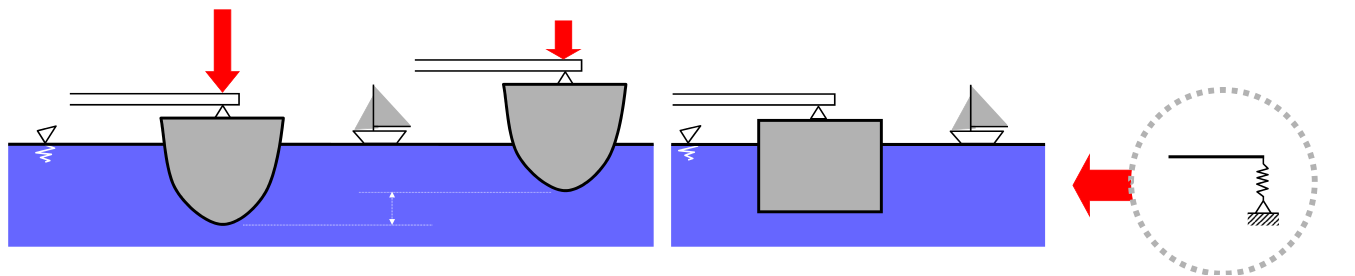
\includegraphics[scale=0.26]{ch2/image4}
		\captionof{figure}{Appui déformable (gauche) et élastique (droite)}
		\end{center}\newpage
		\subsubsection{Appuie élastique}
		Par définition, si le déplacement est \textbf{proportionnel} à la 
		réaction de liaison l'appui est dit élastique. On représente ce 
		bo-goss d’appui par un ressort.\\
				
		De par ces deux définitions, en en déduit que tout appui élastique 
		est forcément déformable, mais pas l'inverse ! \\
		Pour bien finir la section, voici un petit tableau récapitulatif 
		(en 2D!) :
		\begin{center}
		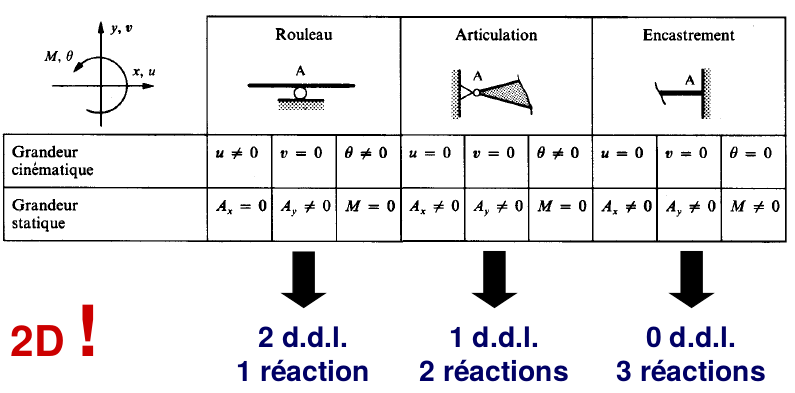
\includegraphics[scale=0.45]{ch2/image1}
		\captionof{figure}{ }
		\end{center}
		Un degré de liberté (d.d.l.) n'est rien d'autre qu'une composante 
		de déplacement libre.
		
\section{Isostaticité - Hyperstaticité}
Avant toute chose, reprenons les deux définitions :
\begin{description}
\item[isostatique]: le problème peut être résolu avec les seules équations 
d'équilibre.
\item[hyperstatique]: il y a plus d'inconnues que d'équations d'équilibre.
\end{description}
Voici un petit tableau pleins d'exemples de nos deux définitions:
\begin{center}
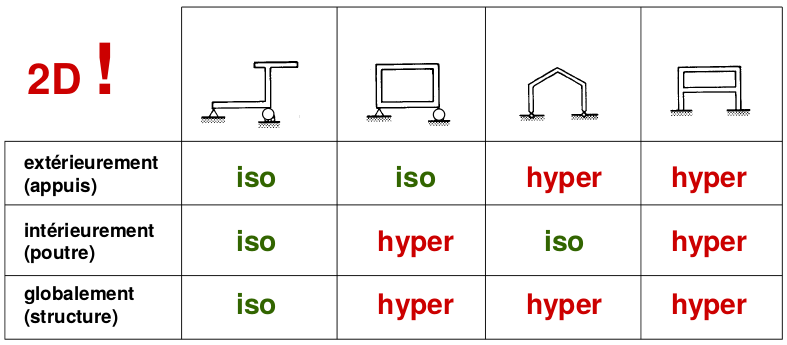
\includegraphics[scale=0.45]{ch2/image2}
\captionof{figure}{ }
\end{center}


\newpage
\section{Théorie des poutres}
	\subsection{La poutre : géométrie}
	\begin{wrapfigure}[5]{r}{4cm}
	\vspace{-5mm}
	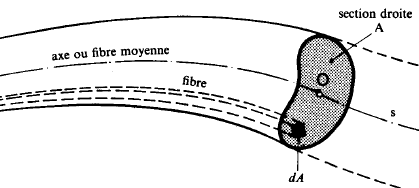
\includegraphics[scale=0.35]{ch2/image3.png}
	\captionof{figure}{ }
	\end{wrapfigure}
	La définition d'une poutre c'est le volume engendré par une surface 
	plane $A$ dont le centre $O$ se déplace le long d'une courbe en 
	restant perpendiculaire à celle-ci. La figure $A$ peut varier mais 
	seulement de façon lente et ses dimensions sont petites comparée à 
	la longueur de la poutre.
	
	
	\subsection{Rappel : notion de contrainte}
	\begin{wrapfigure}[12]{l}{4.5cm}
	\vspace{-5mm}
	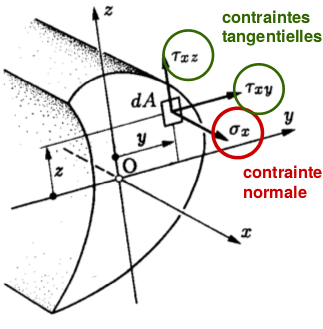
\includegraphics[scale=0.35]{ch2/image5.png}
	\captionof{figure}{ }
	\end{wrapfigure}
	Considérons un volume quelconque que je coupe afin de regarder un 
	élément de surface $dA$ de normale $\vec{n}$. A cause de cette 
	coupe, il apparaît par conservation une force $d\vec{F}$. Or, comme 
	$dA\rightarrow0$, on retrouve bien le vecteur contrainte $\vec{T}^{
	(n)}$ associé à la normale $\vec{n}$ possédant une composante 
	normale $\sigma$ et une composante tangentielle $\tau$.
	\begin{equation}
	\vec{T}^{(n)} = \lim\limits_{dA\rightarrow0} \dfrac{d\vec{F}^{(n)}}{
	dA}\qquad\Longrightarrow\qquad T_i^{(n)} = \tau_{ij}n_j
	\end{equation}
	où $\tau_{ij}$ est le tenseur des contraintes.\\
	La composante tangentielle $\tau$ peut être décomposée selon les 
	axes $x$ et $y$ : $\tau_{xy}$ et $\tau_{xz}$.
	
	\subsection{Poutre : efforts internes (éléments de réduction)}
	\begin{wrapfigure}[8]{r}{3.5cm}
	\vspace{-5mm}
	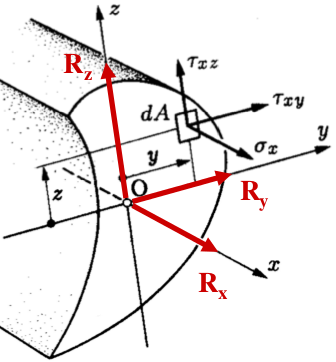
\includegraphics[scale=0.35]{ch2/image6.png}
	\captionof{figure}{ }
	\end{wrapfigure}	
	Comme nous le verrons, les couples et résultantes nous permettrons 
	de "résumer" toutes nos forces/couples en un(e) seul(e) : calculons 
	premièrement nos résultantes :
	\begin{equation}
	\begin{array}{lll}
	\text{Résultante selon $x$ : } & \displaystyle R_x = \int_A\sigma_x\ dA 
	\quad\Rightarrow N; & \text{Effort normal}\\
	\text{Résultante selon $y$ : } & \displaystyle R_y = \int_A\tau_{xy}\ dA 
	\quad\Rightarrow T_y; & \text{Effort tranchant}	\\
	\text{Résultante selon $y$ : } & \displaystyle R_z = \int_A\tau_{zy}\ dA 
	\quad\Rightarrow T_z ;& \text{Effort tranchant}		
	\end{array}
	\end{equation}
	Néanmoins, nous avons coupé notre volume en deux, comment savoir si j'ai 
	pris la partie gauche ou droite ? On se débarrasse de cette ambiguïté en 
	définissant la convention de signe (pour la 2D) présentée sur le schéma 
	ci-contre.\\
	
	Pour le moment résultant, l'idée est la même et il existe également une 
	convention de signe si l'on est en 2D (semblable à celle pour les 
	résultantes mais avec des couples.
	\begin{equation}
	\displaystyle \vec{C} = \int_A\left|\begin{array}{ccc}
	\vec{1_x} & \vec{1_y} & \vec{1_z}\\
	0 & y & z\\
	\sigma_x & \tau_{xy} & \tau_{xz}
	\end{array}\right|\ dA
	\end{equation}
	Ceci nous donne trois moments résultants : 
	\begin{equation}
	\begin{array}{lll}
	\text{Moment résultant selon $x$ : } & \displaystyle C_x = \int_A (
	\tau_{xz}y-\tau_{xy}z)\ dA&\quad\Rightarrow M_x;  \text{Moment de 
	torsion}\\
	\text{Moment résultant selon $y$ : } & \displaystyle C_y = \int_A
	\sigma_xz\ dA&\quad\Rightarrow M_y;  \text{Moment fléchissant}	\\
	\text{Moment résultant selon $z$ : } & \displaystyle C_z = -\int_A
	\sigma_xy\ dA&\quad\Rightarrow M_z;  \text{Moment fléchissant}		
	\end{array}
	\end{equation}
\vspace{-1cm}
\section{Représentations}
	\subsection{Conventions de signes des efforts internes en 2D 
	(éléments de réductions)}
	En 3D on va travailler avec les axes $x,y$ et $z$. Pour se 
	faciliter la tâche, en 2D, on travaille avec $M,N$ et $T$ ainsi 
	que des conventions de signes particulières. Il s'agit des 
	fameux éléments de réductions :\\
	\begin{tabular}{lll}
	$M$ &: moment fléchissant ($M_y$ ou $M_z$); & Positif si les fibres 
	tendues sont "en dessous"\\
	$N$ &: effort normal; & Positif si l'on est en traction\\
	$T$ &: effort tranchant\footnotemark\ 
	($T_y$ où $T_z$); & Positif si la partie de droite descend
	\end{tabular}
	\footnotetext{Souvent noté $V$ dans la littérature.}
	\begin{center}
	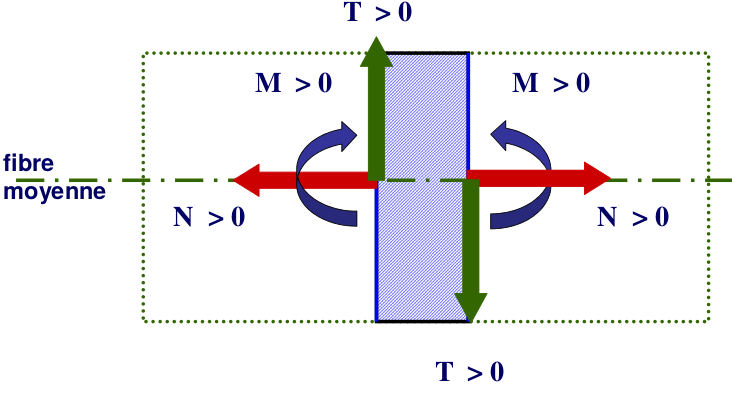
\includegraphics[scale=0.45]{ch2/image7}
	\captionof{figure}{ }
	\end{center}

	Imaginons que  je plie une latte en $U$. La partie supérieure (le 
	creux du $U$) va se mettre en compression et celle du dessous en 
	traction.\\
	\danger Dans ce cours, le \textbf{signe} est aussi important que la 
	valeur numérique !
	
	\subsection{Conventions de représentation des diagrammes $M, N, T$ 
	en 2D}
	\begin{wrapfigure}[9]{r}{6cm}
	\vspace{-8mm}
	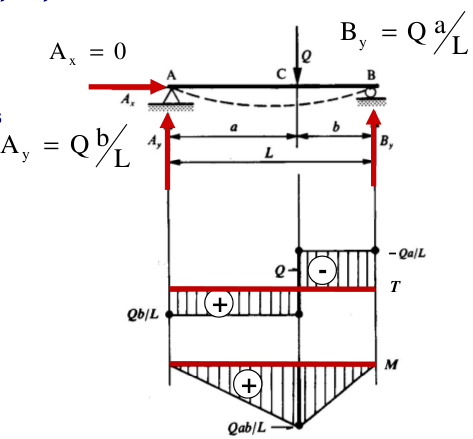
\includegraphics[scale=0.45]{ch2/image8.png}
	\captionof{figure}{ }
	\label{fig:dsctn}
	\end{wrapfigure}	
	Il faut suivre une règle pratique : les valeurs positives du 
	moment fléchissant $M$ (c'est-à-dire si les fibres sont tendues) 
	sont portées \textbf{vers le bas} : le diagramme $M$ est donc 
	forcément porté du côté des fibres tendues, pas besoin de préciser 
	d'autres conventions. Pour uniformiser le tout, on dessine les autres 
	diagrammes avec des valeurs positives vers le bas. Histoire d'être 
	sur, on rajoute dans les diagramme un plus ou un moins, indiquant 
	le signe de la résultante. Il existe d'autres moyen d'indiquer 
	le signe : voir TP et slides 29-30. \\
	
	\textsc{Explications complémentaires sur la \autoref{fig:dsctn}} : \\
	La première chose est de savoir que l'axe $y$ de la figure du 
	diagramme du corps libre et vers le haut, alors que dans le 
	$M,N,T$ il est axé vers le bas. Par \textbf{convention}, on dit 
	que la partie de droite \textit{descend} impliquant, selon la 
	règle pratique, que $T>0$. Si l'on fait une coupure à droite de 
	$C$, le bilan des forces$_y$ s'écrit $T=-B_y$, d'où le signe 
	négatif sur le diagramme $M,N,T$.\\
	Autre astuce : si on a une force vers le haut sur le DLC, il 
	suffit de "descendre" (aller vers le haut) de la valeur de cette 
	force pour le diagramme de $T$ (comme avec $B_y$). Pour respecter 
	ces conventions, on commence à tracer ces diagrammes par la 
	droite.\\
	
	La grande question est de savoir qu'est ce qu'on appelle "haut" 
	et "bas". Par \textbf{convention}, on le définit de la façon 
	suivante (et même un exemple en prime, à droite):
	\begin{center}
	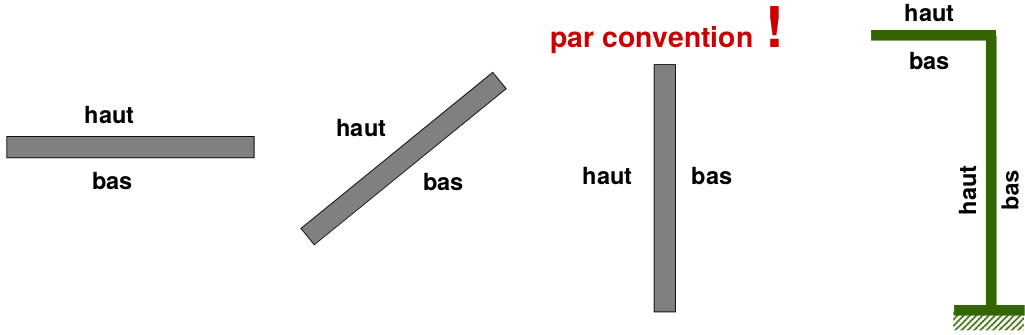
\includegraphics[scale=0.30]{ch2/image9}
	\captionof{figure}{ }
	\end{center}
	Résumons brièvement ce que nous venons de définir :
	\begin{itemize}
	\item[$\bullet$] Les conventions pour $M,N,T$ ne nécessite pas 
	l'utilisation de système d'axe, ni même de préciser si l'on 
	travaille avec la partie "gauche" ou "droite".
	\item[$\bullet$] Ces conventions sont liées au comportement 
	structural.
	\item[$\bullet$] Ces conventions ne sont pas cruciales, 
	l'important est dans l'interprétation du diagramme pour la 
	compréhension du comportement structural.
	\end{itemize}\ \\
	
	\begin{wrapfigure}[8]{l}{11cm}
	\vspace{-10mm}
	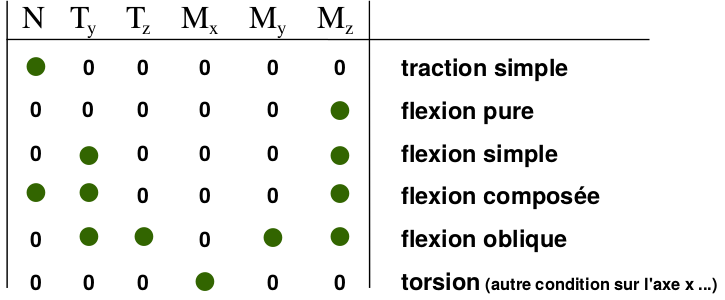
\includegraphics[scale=0.45]{ch2/image10.png}
	\captionof{figure}{ }
	\end{wrapfigure}
	Il existe évidemment plein de conventions, mais celles-ci sont 
	les plus couramment utilisées. Elles nous permettront de 
	traiter tous les cas figurant dans le tableau ci-contre (l'objet 
	des prochains chapitres).
	
	\newpage
	
\section{Revenons à notre poutre}
	\subsection{Poutre rectiligne en 2D : relation $T \leftrightarrow 
	q(x)$}
	\begin{wrapfigure}[9]{l}{4.5cm}
	\vspace{-5mm}
	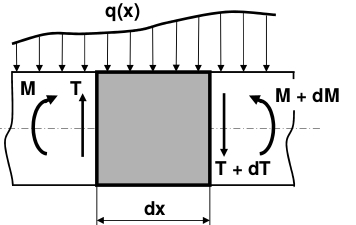
\includegraphics[scale=0.35]{ch2/image11.png}
	\captionof{figure}{ }
	\end{wrapfigure}
	On cherche à lier notre effort tranchant $T$ à une charge 
	répartie. Considérons un morceau de quelque chose et regardons ce 
	qui agit dessus : un moment fléchissant ainsi qu'un effort 
	tranchant. Si je considère l'équilibre de translation vertical :

	\begin{equation}
	-T + q(x)\ dx + (T+dT) = 0\qquad\Longrightarrow \qquad \dfrac{dT}{dx}
	=-q(x)
	\end{equation}
	Cette précieuse relation nous informe que si nous avons un tronçons 
	sur laquelle je n'ai pas de charge répartie, $dT/dx = 0$ impliquant 
	que l'effort tranchant est constant. Ceci est vrai en 3D, pour autant 
	que l'on considère des axes cohérents.\\
	\danger Retenir que l'effort tranchant est proportionnel à la charge 
	et ensuite regarder sur le dessin pour le signe.
	\subsection{Poutre rectiligne en 2D : relation $M \leftrightarrow T$}
	\begin{wrapfigure}[9]{r}{4cm}
	\vspace{-5mm}
	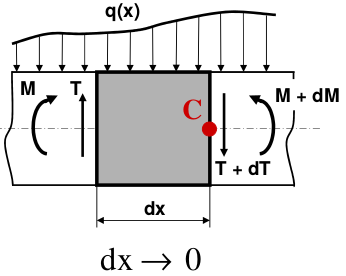
\includegraphics[scale=0.35]{ch2/image12.png}
	\captionof{figure}{ }
	\end{wrapfigure}
	Cette fois-ci, je vais écrire l'équilibre de rotation autour du 
	point $C$. Le choix de ce point est arbitraire, mais $C$ permet de 
	se débarrasser du $T+dT$. Nous avons donc
	\begin{equation}
	M + T\ dx - q(x)\ dx \frac{dx}{2} - (M+dM)=0\qquad\Longrightarrow\qquad
	\dfrac{dM}{dx}= T
	\end{equation}
	En effet, les $M$ s'annulent et le produit de $dx$ tend plus rapidement 
	vers 0 que le reste. Ceci à pour conséquence que le moment fléchissant 
	est \textbf{extrémum} si $T$ est nul. Il s'agit bien évidemment d'une 
	relation linéaire et les conditions pour passer en 3D sont les mêmes.
	
	
	\subsection{Conséquences pour les diagrammes $M$ et $T$ en 2D}
	Si il n'y a pas de charge répartie ($q(x)=0$), l'effort tranchant $T$ est 
	constant et le moment fléchissant $M$ varie linéairement (degré 1). Si 
	par contre il y a répartition de charge uniforme ($q(x)=cste$), $T$ varie 
	linéairement et $M$ quadratiquement.\\
	
	Si la charge est concentrée ($P$), l'effort tranchant sera discontinu et la 
	dérivée du moment fléchissant le sera également (la pente de $M$ sera 
	discontinue) :
	\begin{equation}
	T_{gauche} - T_{droite} = P
	\end{equation}
	Cette discontinuité est bien celle que nous avions observée pour $T$ sur 
	la \autoref{fig:dsctn}.\\
	
	\textsc{Exemples} : voir slides 40-44.
\newpage
\section{Démarches en résistances des matériaux}
	\subsubsection{Démarches}
Il existe deux méthodes en RDM :
\begin{enumerate}
\item Méthode \textit{inverse}
\begin{itemize}
\item[$\bullet$] Postule une distribution de contrainte
\item[$\bullet$] Déduit les éléments réduction
\item[$\bullet$] Calcule les déformations
\item[$\bullet$] Vérifier que les équations de compatibilité sont bonnes (!!)
\end{itemize}

\item Méthode \textit{cinématique}
\begin{itemize}
\item[$\bullet$] Postule un champ de déplacement
\item[$\bullet$] Calcule les déformations
\item[$\bullet$] Calcule les contraintes
\item[$\bullet$] Calcule les éléments de réduction
\item[$\bullet$] Relation contraintes $\leftrightarrow$ éléments de 
réduction : equations de compatibilité automatiquement vérifiées (!!)
\end{itemize}
\end{enumerate}
	
La première méthode est intuitive, mais on ne peut pas déduire clairement 
ce qui est valable ou pas. La seconde est systématiques mais permettent de 
voir directement ce qui dépend du matériau.
	
	\subsubsection{Équations de compatibilité}
	Ces équations expriment
	\begin{itemize}
	\item[$\bullet$] Les déplacements par un vecteur (3 composantes)
	\item[$\bullet$] Les déformations par un tenseur (6 composantes)
	\item[$\bullet$] On obtient ces 6 composantes par dérivées des 
	3 composantes du vecteur
 	\item[$\bullet$] Si on part des déformations : les 3 composantes 
 	doivent s'obtenir par intégration des 6 composantes des déformations
	\item[$\bullet$] Si on part des déplacement, il suffit de calculer 
	les dérivées ad-hoc.
	\end{itemize}
	
	
	
	
	
	
	
	
	
	
	
	
	
	
	
	
	
	
	
	
	
	
	
	
	
	
	
	
	
	
